The demonstration setup is depicted in Figure~\ref{fig:demo}. The demonstration mimics a use case in public transportation, whereby data on connected vehicles are collected and aggregated at some fog nodes (which estimate the traffic intensity in a given region).
We use real-world data on connected vehicles, covering $245,369$ vehicles moving across Italy. Data consists of vehicle location, the timestamp of the event created, engine status and type of the vehicle. Events are created converting their recorded timestamp into real-time. On average, $0.8$ events are generated per millisecond.
%DM - taking this out, need to get clearance from Otonomo first
% The raw data is provided by our technology partner Otonomo~\footnote{https://otonomo.io/}.
The processing component implements the following functionality: It filters the incoming traffic by their recorded region and sends aggregated results every 10 seconds to the cloud.
On the cloud tier, we deploy the Telegraf, InfuxDB and Grafana (TIG) stack to receive and visualize aggregated results. The dashboard is shown in Figure~\ref{fig:dashboard}.
% To illustrate the overall architecture and its benefits, we demonstrated the following:
% \paragraph{IoT data generation}
% We simulated IoT traffic using real-life vehicle traffic data recorded throughout Italy.
% \paragraph{Flink Job}
% Processed data pushed every 10 second to custom topic of MQTT broker.
% \paragraph{Monitoring data in a cloud}
% On Cloud environment, we deployed Telegraf, InfuxDB and Grafana (TIG) stack to receive and visualize aggregated results via custom MQTT topic from Fog MQTT broker.
The platform was able to tolerate the traffic without showing any backpressure
while maintaining available processing space for other tasks.


\begin{figure}[htbp]
\centerline{
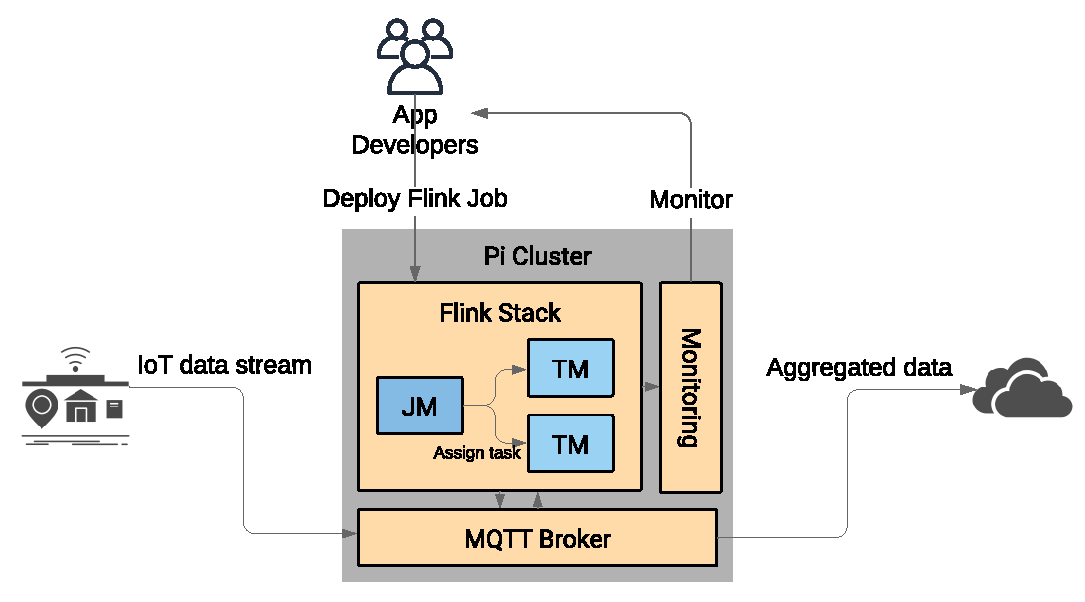
\includegraphics[width=1\linewidth]{figures/fog_activity.pdf}}
\caption{Demonstration setup}
\label{fig:demo}
\end{figure}

\begin{figure}[htbp]
\centerline{
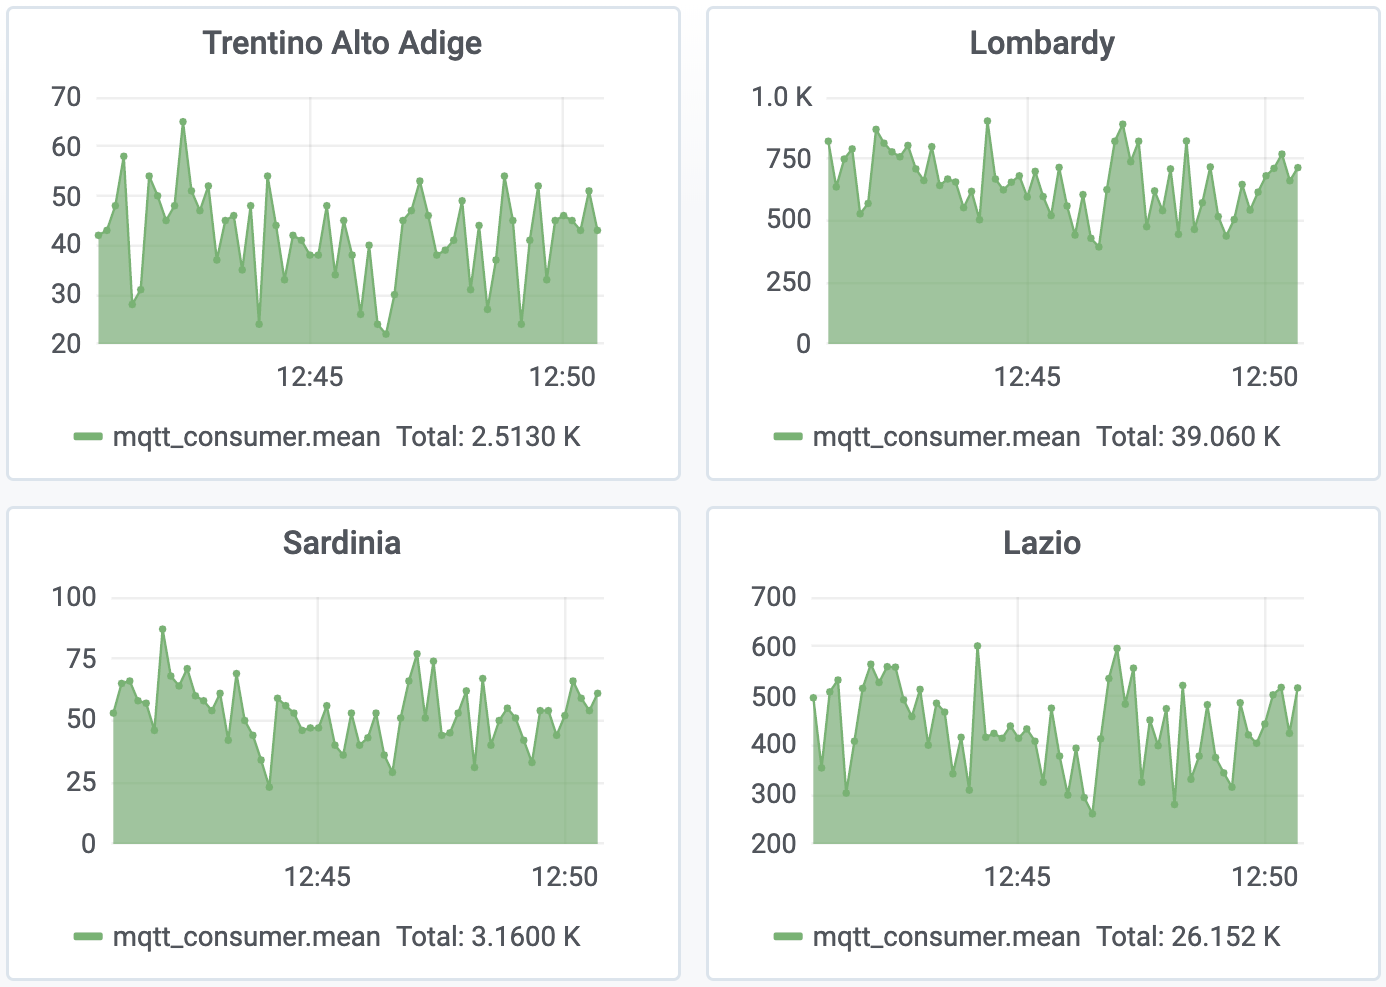
\includegraphics[width=1\linewidth]{figures/fog_dashboard_big.png}}
\caption{Demonstration: the cloud dashboard for traffic monitoring at the regional level.}
\label{fig:dashboard}
\end{figure}


